\documentclass[a4paper, 11pt]{article}
\usepackage{fullpage} % changes the margin
\usepackage[spanish]{babel}
\usepackage[utf8]{inputenc}
\usepackage{url}
\usepackage[sort&compress, numbers]{natbib}
\usepackage{graphicx}

\begin{document}
\begin{center}
\LARGE \bf Tarea Nº 0\\ Simulaci\'on
\end{center}

\bigskip

\hfill\textbf{Nombre:} José Adrián García fuentes\hfill
\hfill\textbf{Profesor:} Satu Elisa Schaeffer\hfill \\
\textbf{Fecha} 10/febrero/2021\\

\hrule

\bigskip
\begin{abstract}
Simple demo explicando uso basico de \LaTeX{} en overleaf.
    
\end{abstract}
\hrule

\section{Introducción}

\medskip

\bigskip

 {Este es un texto ejemplo con la finalidad de ir aprendiendo el uso corrector de overleaf, de la materia de simulacion de nanomateriales el presente trabajo sera subido a un repositorio de github}
 
\vspace{1cm}

Ademas en el presente trabajo aprenderemos a citar fuentes de la siguiente manera \citep{ejemplo} los datos completos de esta cita se encuentran en el apartado de referencias.
\vspace{1cm}

Generar tablas de datos como la numero \ref{datos} al final de esta hoja Een la que se muestra una relacion  de alumnos y maestros de la clase de simulacion. O bien agregar figuras o imagenes. como la FIG \ref{nanobots} que muestra un nanobot postrado en una celula sanguinea.

\section{Conclusiones}
Aun se tienen dudas del uso pero seguiremos practicando.

\begin{table}[b]
    \caption{CUADRO RELACION ALUMNOS MAESTRO DE SIMULACION}
    \label{datos}
    \centering
    \begin{tabular}{c|cr}
    ALUMNOS     &  4\\
    MAESTROS     &  1
    \end{tabular}
\end{table}


\begin{figure}[b]
    \centering 
    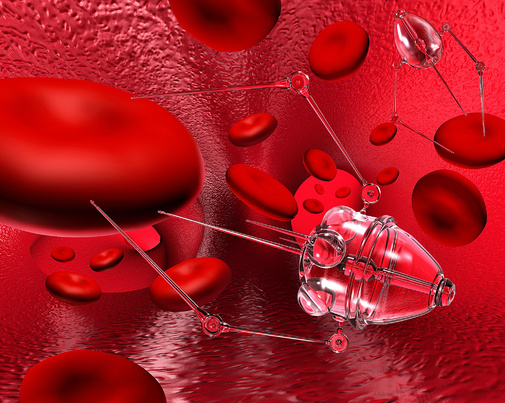
\includegraphics[width=70mm]{nanobots.jpg}
    \caption{\label{fig1}
    \label{nanobots}}
\end{figure}

\bibliography{simu}
\bibliographystyle{plainnat}





\end{document}
